\cleardoublepage

\chapter{Aplicación Android}
\label{makereference6}

La parte del servidor Bluetooth se ha implementado sobre la plataforma Android. La principal razón por la que optamos por esta plataforma es la de que para programar una aplicación en iOS es necesario disponer de un ordenador Macintosh, condición que no cumplíamos, y debido a que de los tres componentes del grupo, dos teníamos disponible un dispositivo Android, nos pareció un paso lógico.

Hay numerosos frameworks disponibles para programar aplicaciones Android, pero nos decantamos por la herramienta que ofrece Google, Android Studio, que al estar basado en la plataforma Eclipse nos resultó familiar, a la vez que proveía muchas funcionalidades específicas para Android.

Una aplicación Android se implementa en Java para especificar la funcionalidad y en XML para estructurar la parte gráfica. Aunque tuvimos que familiarizarnos con el modo de gestionar las vistas en Android, el hecho de basar la funcionalidad en Java nos ha facilitado desarrollar rápidamente aplicaciones sencillas para probar funcionalidades y, eventualmente, la aplicación final. 

Hemos basado el diseño en el patrón Modelo-Vista-Controlador, comunicando la vista y la funcionalidad mediante comandos. En la siguiente imagen se muestra un diagrama de clases para ver cómo hemos estructurado el código de la app.

\begin{figure}[h]%t=top, b=bottom, h=here
	\centering
    \includegraphics[scale=0.5]{figures/diagrama_clases_general.png} % TODO hacer que esto no quede horrible
    \caption[Diagrama de clases general de la aplicación Android]{Diagrama de clases general de la aplicación Android}
   	\label{figuraDiagramaClasesGeneral}
\end{figure}

\section{Front-End}
\label{makereference6.1}

Para la interfaz de usuario, hemos implementado una actividad principal, que se mantiene estática durante toda la vida de la aplicación, con fragmentos que se van cargando dentro de ésta. La actividad principal mantiene una barra de título en la parte superior que se encuentra siempre presente en la que hemos añadido un menú Hamburger, que permite desplegar una lista con accesos directos a las opciones de la app, bien pulsando sobre el icono o deslizando el dedo de izquierda a derecha. Este diseño es muy utilizado en apps Android.

\begin{figure}[h]%t=top, b=bottom, h=here
	\centering
    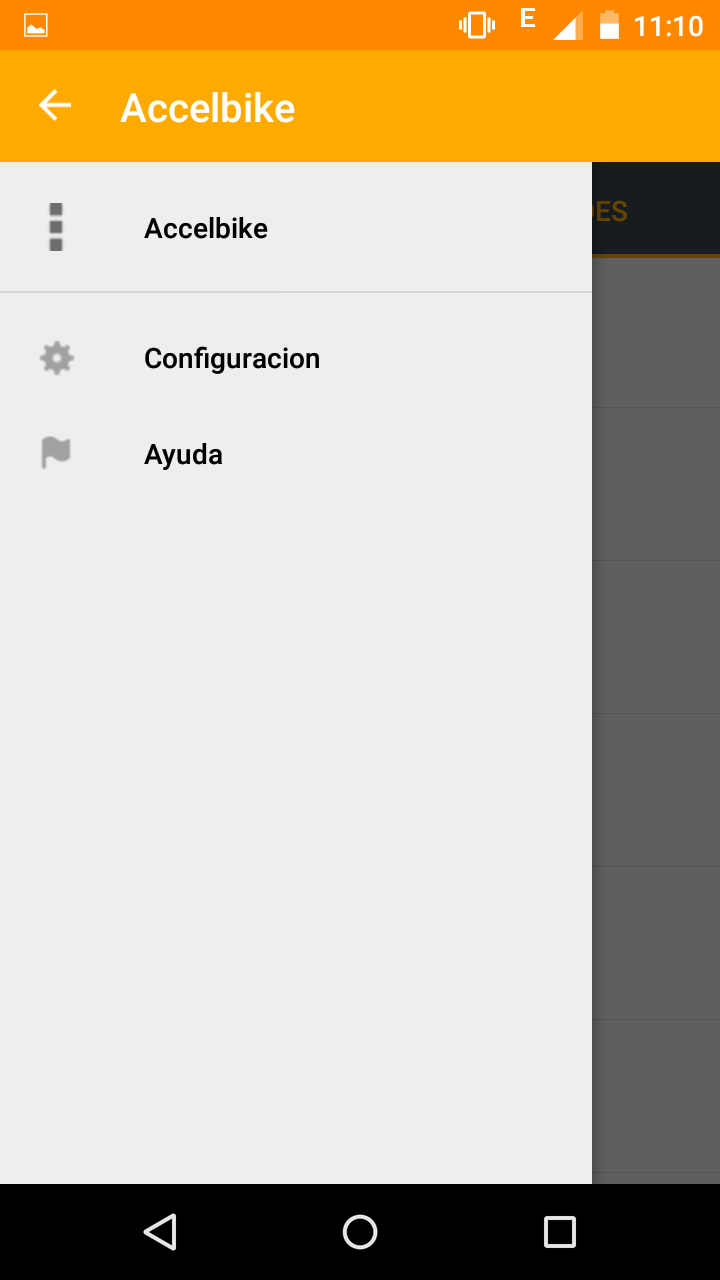
\includegraphics[scale=0.2]{figures/app_menu_deslizable.png} % TODO hacer que esto no quede horrible
    \caption[Menú deslizable de la aplicación Android]{Menú deslizable que aparece al pulsar en el botón de menú o al deslizar de izquierda a derecha}
   	\label{figuraAPPMenu}
\end{figure}

A continuación explicaremos en detalle los fragmentos que se cargan en la app.

\subsection{Vista principal}
\label{makereference6.1.1}

La primera pantalla que aparece al iniciar la aplicación. Está dividida en dos pestañas, sesión y actividades, lo que facilita acceder a las funcionalidades principales de la app. La pestaña que aparece por defecto es la de sesión, que es la que lleva a cabo el objetivo principal de este proyecto, ya que permite iniciar la recogida de datos del acelerómetro y del GPS. La forma de llevar a cabo esta funcionalidad se explicará más adelante.

\begin{figure}[h]%t=top, b=bottom, h=here
	\centering
    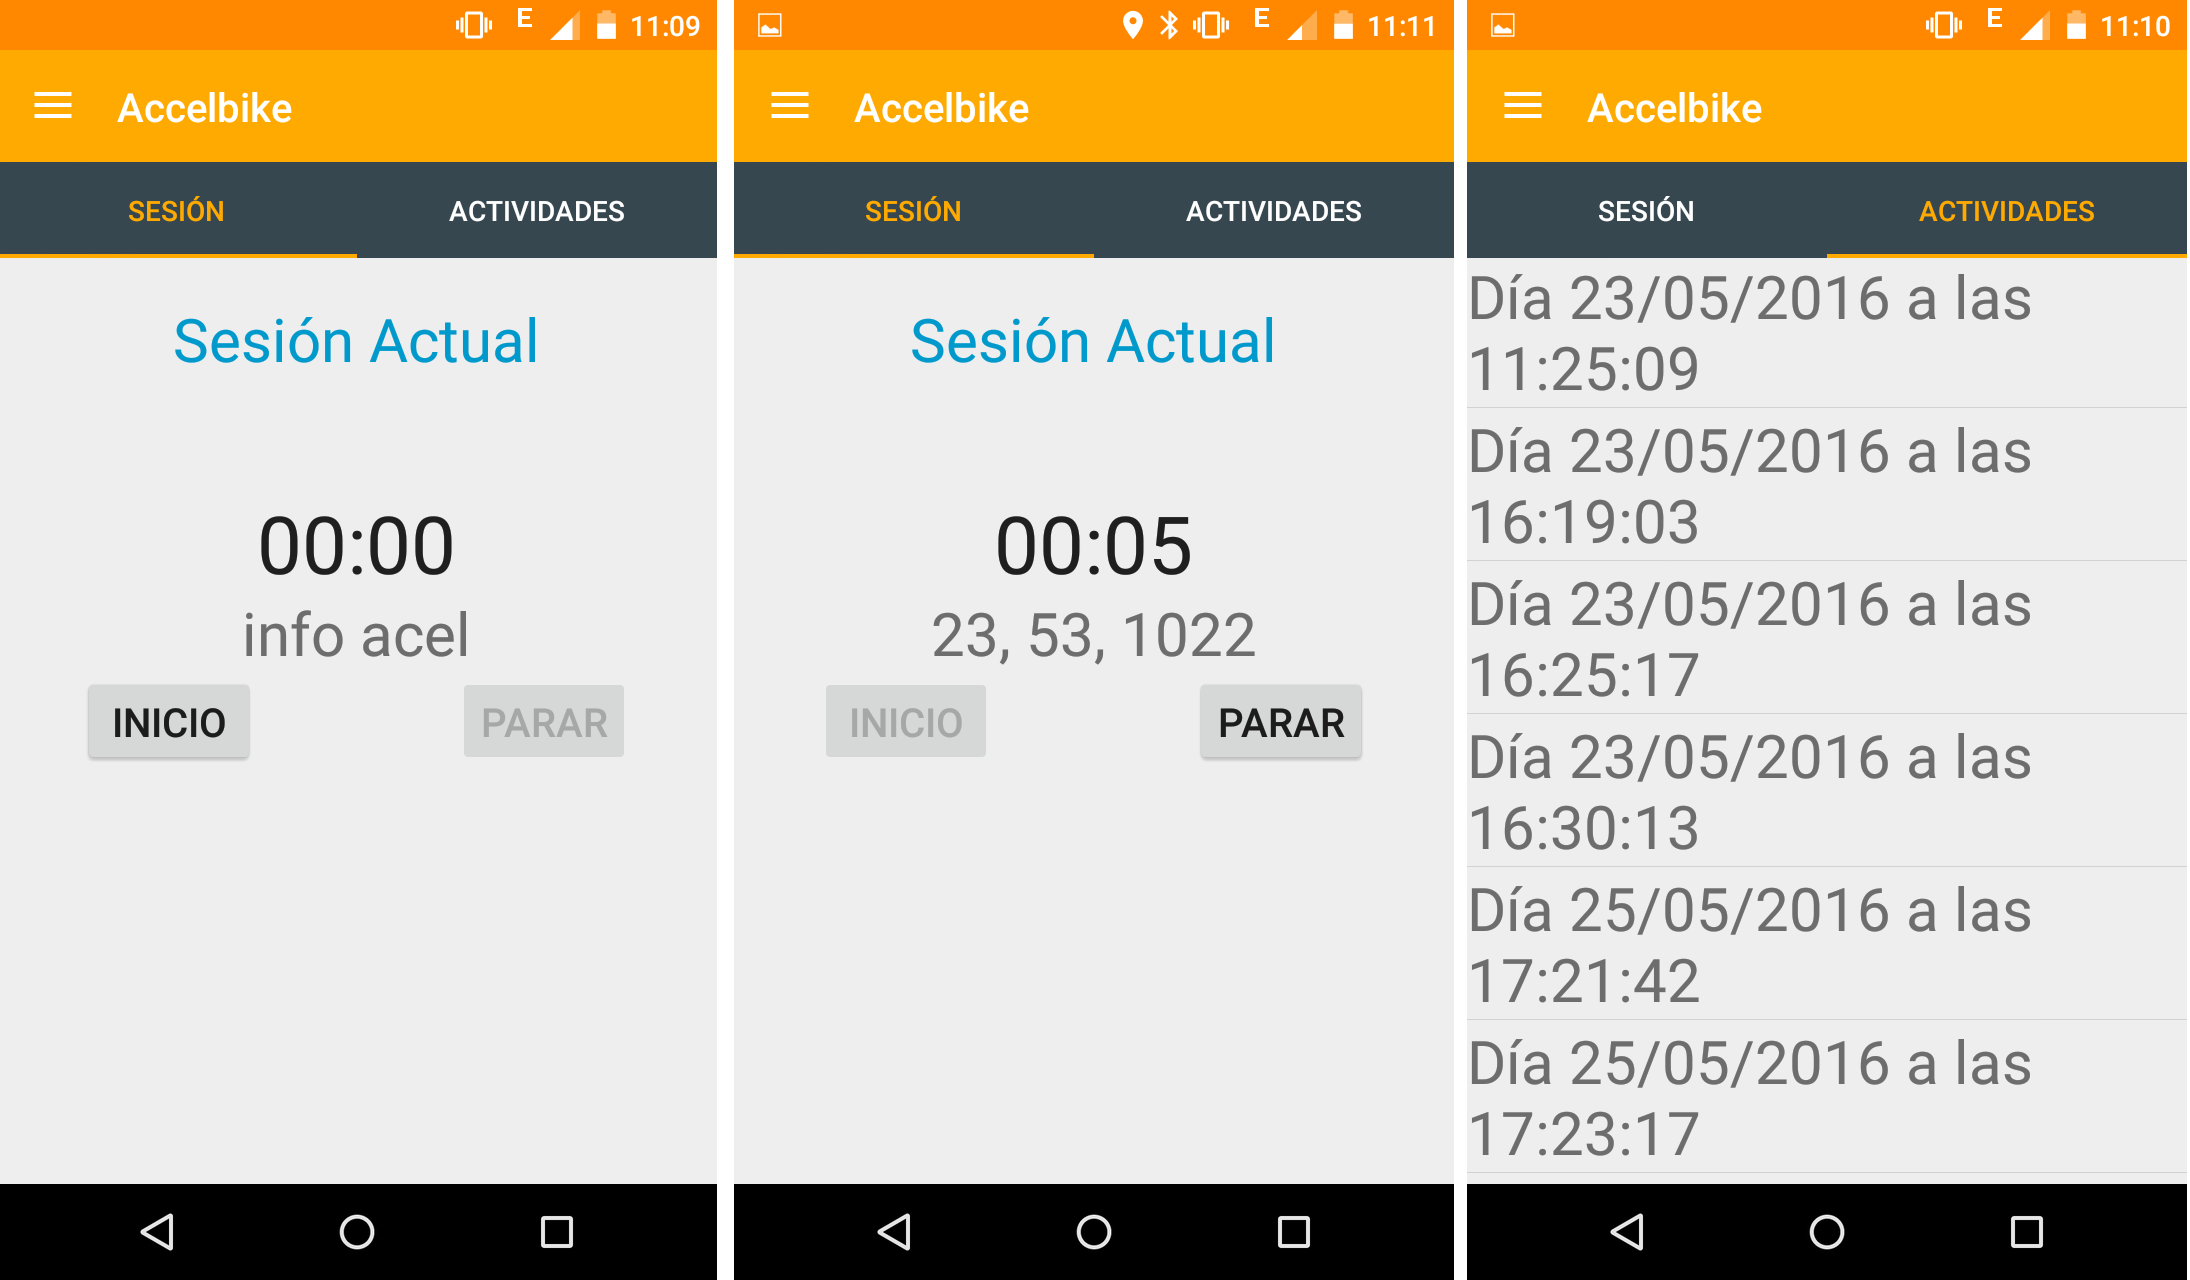
\includegraphics[width=\linewidth]{figures/app_tabfragment.png} % TODO hacer que esto no quede horrible
    \caption[Vista principal de la app Android]{Vista principal de la app. De izquierda a derecha: Sesión sin iniciar, Sesión iniciada y Vista de sesiones}
   	\label{figuraAPPPrincipal}
\end{figure}

En esta pestaña de sesión tenemos dos botones, inicio y parar, un cronómetro y un espacio en el que se nos va a mostrar la información de acelerometría recibida.

La segunda pestaña a la que se puede acceder es la de actividades, que muestra una lista de todas las sesiones guardadas. El nombre nos muestra el día y hora a la que se realizó. Pulsando en cada una de estas actividades lanza un fragmento con los datos de la ruta.


\subsection{Configuración y Ayuda}
\label{makereference6.1.2}

En la pantalla de configuración (Figura~\ref{figuraAPPConfigAyuda}) se permite al usuario realizar la conexión con la placa. Para ello contiene un botón para escanear los dispositivos BLE cercanos, que aparecerán en una lista en la zona inferior, y al pulsar en uno de los elementos de esta lista nos conectaremos y así podremos comenzar la sesión.

\begin{figure}[h]%t=top, b=bottom, h=here
	\centering
    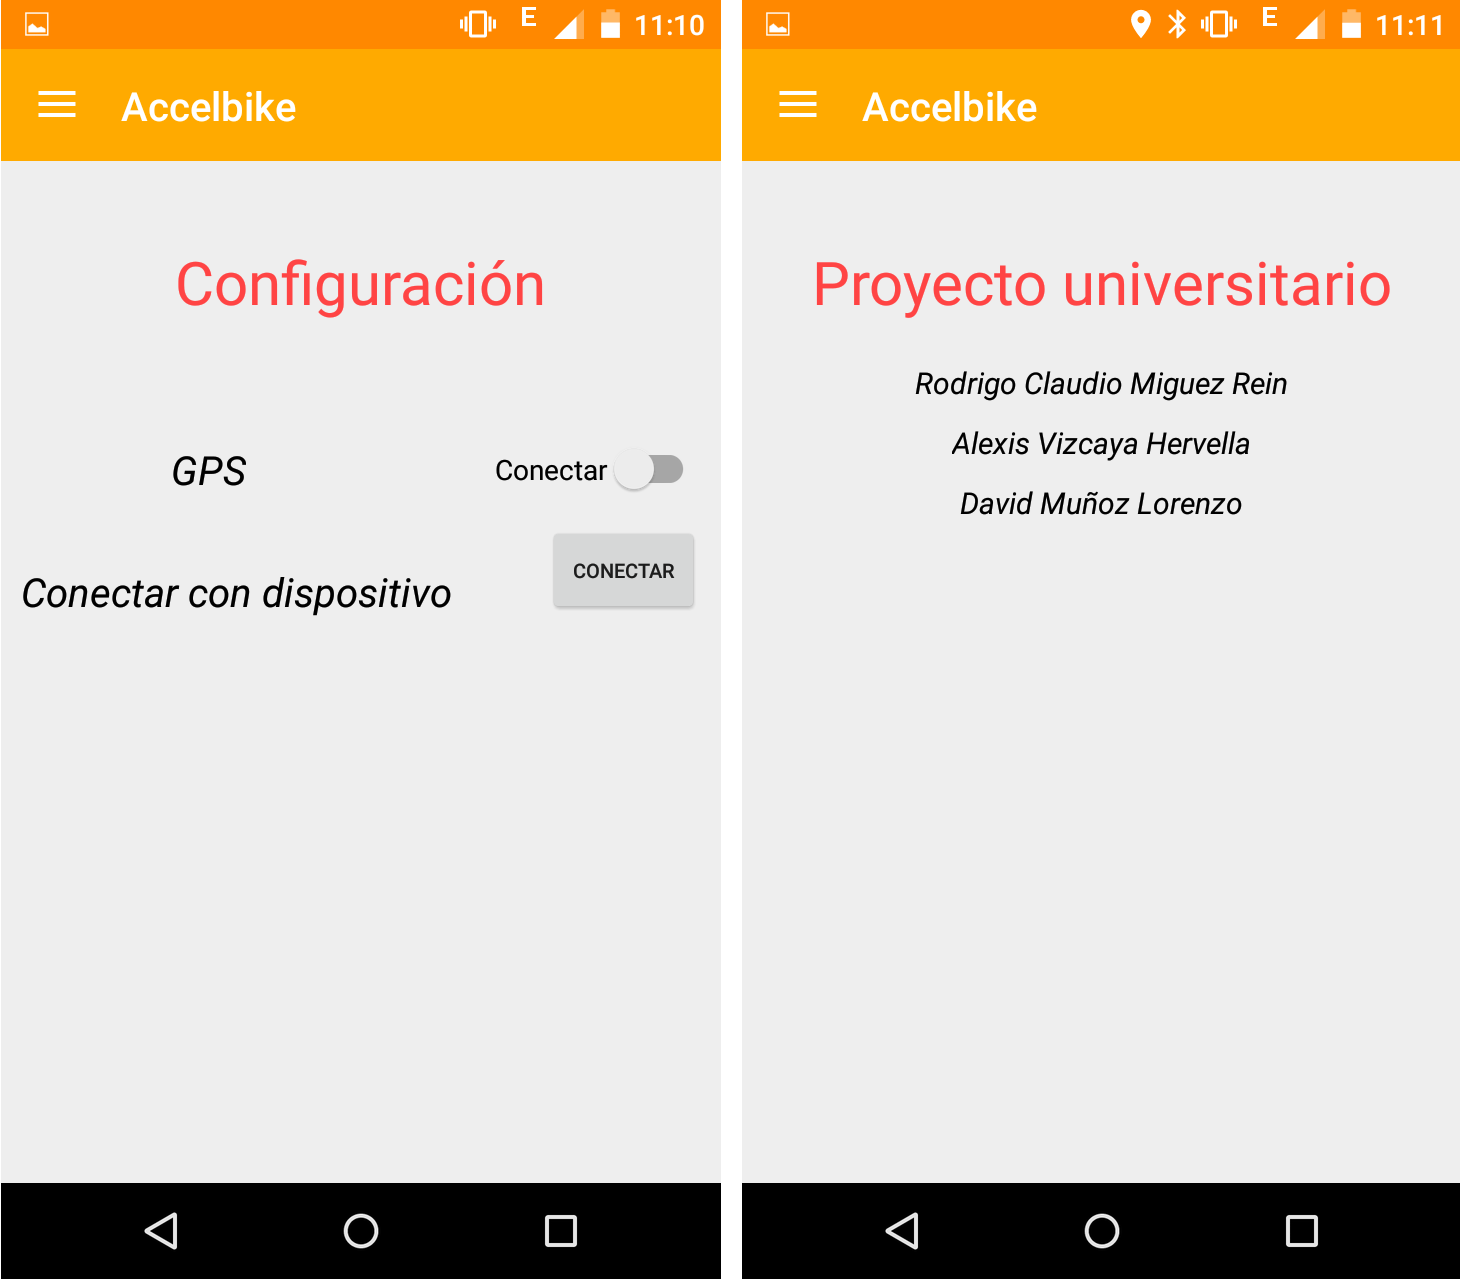
\includegraphics[scale=0.2]{figures/app_config_ayuda.png} % TODO hacer que esto no quede horrible
    \caption[Vista de configuración y de ayuda]{Vistas de Configuración y Ayuda}
   	\label{figuraAPPConfigAyuda}
\end{figure}

\subsection{Vista resumen de sesión}
\label{makereference6.1.3}

Esta vista se lanza cuando terminamos una sesión (botón parar), o cargamos una actividad desde la pestaña de actividades. En ella se muestra un mapa con la ruta realizada, la cual se colorea según la aceleración producida en cada momento. También nos muestra el tiempo, la distancia recorrida y la velocidad media del trayecto. En la Figura~\ref{figuraAPPSesion} se muestra un ejemplo de la vista con una ruta realizada alrededor de la Facultad de Informática.

\begin{figure}[h]%t=top, b=bottom, h=here
	\centering
    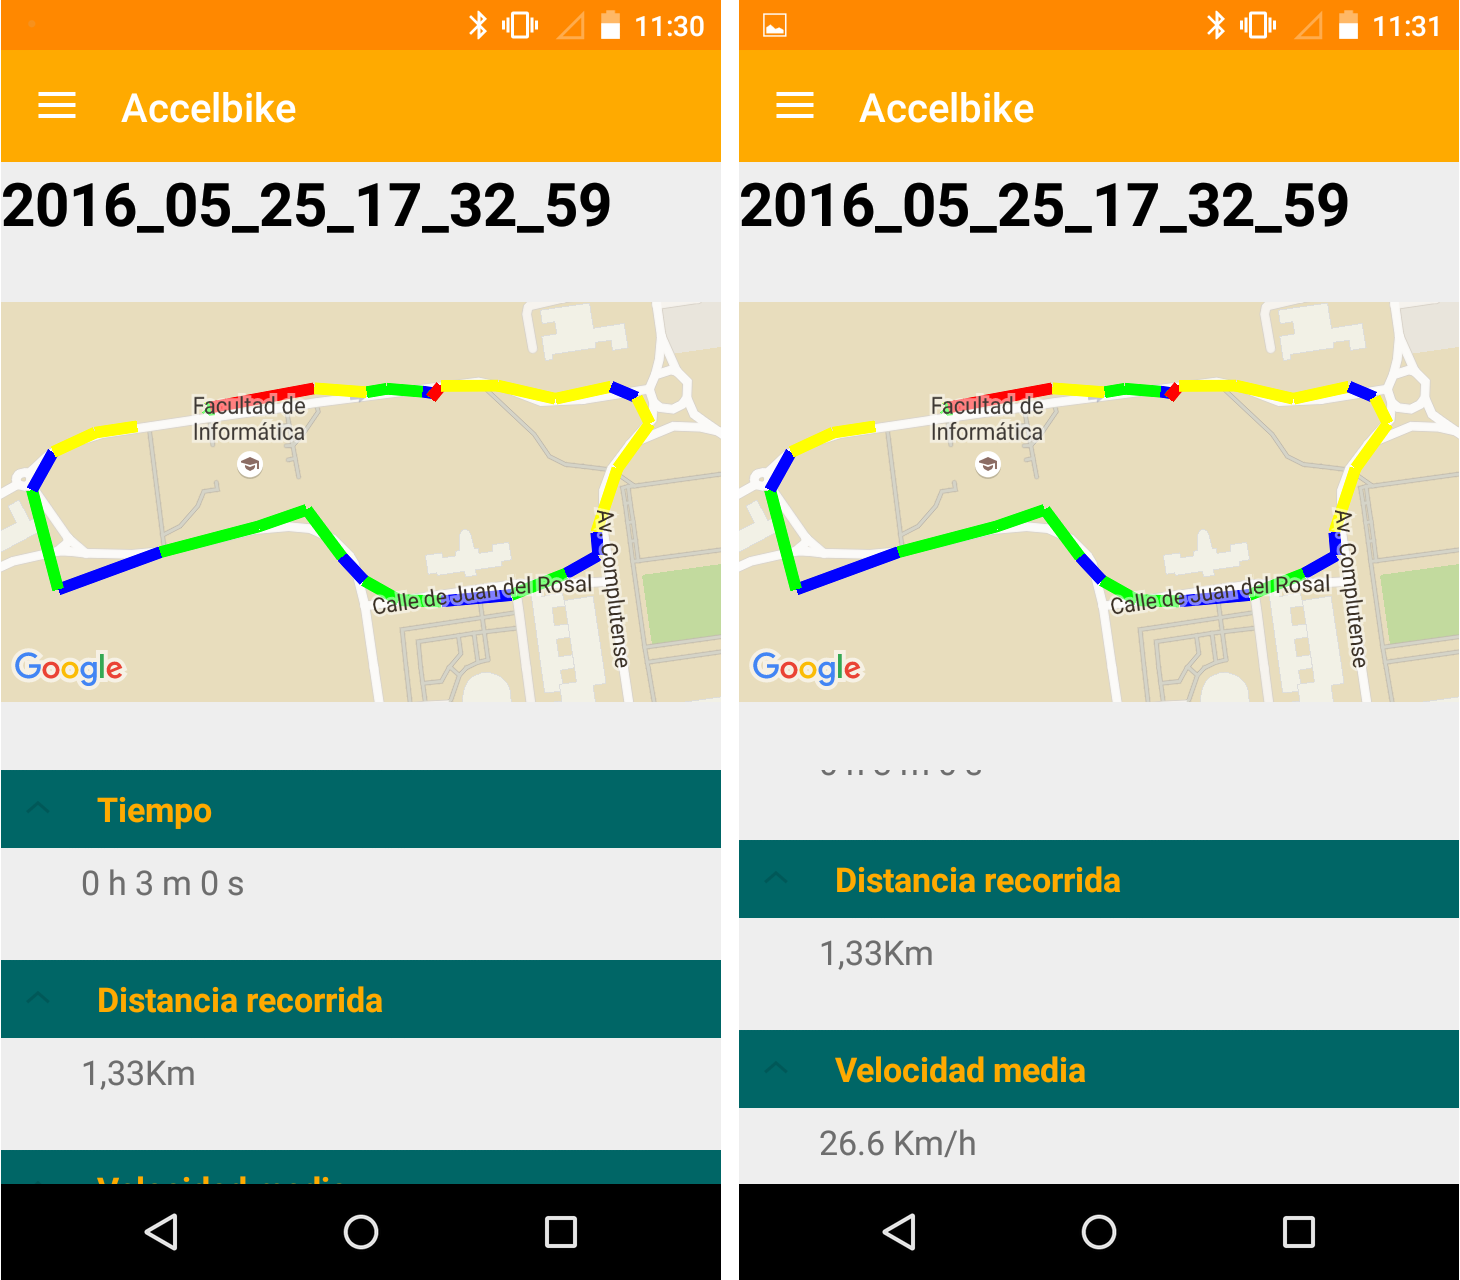
\includegraphics[scale=0.2]{figures/app_resumen_sesion.png} % TODO hacer que esto no quede horrible
    \caption[Vista de resumen de sesión]{Vista de Resúmen de Sesión. Se muestra la ruta y la información recogida.}
   	\label{figuraAPPSesion}
\end{figure}

\section{Funcionamiento}
\label{makereference6.2}

A continuación describiremos la funcionalidad de los casos de uso más importantes de la aplicación, detallando la estructura de clases utilizada.

\subsection{Conexión al dispositivo BLE}
\label{makereference6.2.1}

\begin{figure}[h]%t=top, b=bottom, h=here
  \centering
    \includegraphics[scale=0.5]{figures/diagrama_clases_ble.png} % TODO hacer que esto no quede horrible
    \caption[Diagrama de las clases que intervienen en una conexión BLE]{Diagrama de las clases que intervienen en una conexión BLE}
    \label{figuraDiagramaClasesBLE}
\end{figure}

Para realizar la comunicación entre la placa y el móvil, primero debemos escanear los dispositivos BLE cercanos. Para ello utilizamos una clase de la API de Android llamada \textit{BluetoothLeScanner}, que busca exclusivamente dispositivos Bluetooth Low Energy y nos devuelve la información recogida en los paquetes de anuncio sobre los dispositivos en forma de \textit{BluetoothDevice}.

Una vez obtenidos, los mostramos en forma de lista en la que aparece el nombre de cada dispositivo, como se muestra en la Figura~\ref{figuraAPPConfigAyuda}, para que el usuario elija a cuál se quiere conectar. 

Hemos creado una clase \textit{BLEGatt}, que es la que se encarga de mantener la información del enlace. Para establecer la conexión, se hace uso de esta clase, que configura el GATT para empezar a explorar los servicios, como se explicará más adelante.

\subsection{GPS}
\label{makereference6.2.2}

Android por motivos de seguridad no permite activar el GPS del móvil desde una app, por lo que lo único que hacemos es avisar al sistema operativo para que abra la ventana de configuración de la ubicación.
Una vez activado, la API de Android nos ofrece una clase llamada \textit{LocationManager}, que nos permite establecer un período de actualización, de modo que guarda de manera regular la última localización conocida, a la que podemos acceder.

\subsection{Funcionamiento durante la marcha}
\label{makereference6.2.3}

\begin{figure}[h]%t=top, b=bottom, h=here
  \centering
    \includegraphics[scale=0.5]{figures/diagrama_clases_marcha.png} % TODO hacer que esto no quede horrible
    \caption[Diagrama de las clases que intervienen en una sesión]{Diagrama de las clases que intervienen en una sesión}
    \label{figuraDiagramaClasesMarcha}
\end{figure}

Para llevar a cabo una sesión tenemos tres clases, como se puede ver en la Figura~\ref{figuraDiagramaClasesMarcha}, que heredan de Thread: BluetoothThread, CoordenadasThread y FileThread. De ese modo, la lectura de los datos del acelerómetro, los datos de la ubicación y la escritura en el archivo se hacen de manera independiente.\\

\textbf{BluetoothThread} utiliza la clase BLEGatt explicada anteriormente para leer las características recibidas. Como se menciona en la Sección~\ref{makereference5.2}, hemos configurado la placa nRF51-DK para que tenga un servicio con UUID 0xA000, que contiene la característica con UUID 0xA001, que es la que nos interesa para obtener la información del acelerómetro. Para descubrir este servicio, se puede realizar lo que se llama \textit{escaneo de servicios}, que devuelve una lista de los servicios del dispositivo, pero como ya conocemos de antemano el UUID, podemos acceder a él directamente.

Para recoger la información del acelerómetro, se accede la característica mencionada a través de su identificador, lo que devuelve una clase de Android llamada \textit{BluetoothGattCharacteristic}, que podemos usar para leer el valor del GATT.\\

\textbf{CoordenadasThread} accede periódicamente a la última localización guardada en \textit{LocationManager}, como se explicaba en la sección anterior.\\

\textbf{FileThread} se encarga de lanzar los dos hilos de BluetoothThread y CoordenadasThread y, periódicamente, recoge los datos obtenidos por ambos. Estos son guardados mediante una clase llamada FileManager que es la encargada del manejo de archivos. El formato del archivo que se crea consiste en una línea por cada muestreo dividida de la siguiente manera:

\begin{center}
(latitud);(longitud);(coordenadaX);(coordenadaY);(coordenadaZ)
\end{center}

con una última línea indicando el tiempo total de la sesión de la siguiente manera: 

\begin{center}
T(tiempo en milisegundos)
\end{center}

Este archivo se guarda en una carpeta en el almacenamiento externo del móvil llamada accelbike; si no existe dicha carpeta, la clase se encarga de crearla.

Para detener la sesión aprovechamos una característica de los hilos en Java que nos permite diferenciarlos de manera única a través de un nombre dado por una cadena de caracteres. De este modo podemos detener un determinado hilo a través de este nombre, por lo que basta con finalizarlos para que se termine la sesión.

\subsection{Generación de mapas tras marcha}
\label{makereference6.2.4}

Una vez hemos terminado una sesión, o bien hemos cargado una sesión anterior desde la vista de actividades, volvemos a llamar a la clase FileManager, esta vez para cargar el archivo. Se parsea el archivo y se agrupan las localizaciones de dos en dos calculando la distancia entre ellas y creando una polilínea a la que se le da color con los datos del acelerómetro. Cada polilínea se guarda en un array, que junto el tiempo y la distancia se inserta en una clase que actúa como Transfer. Este transfer se devuelve a la vista MapFragment, que se encarga de mostrar los datos de velocidad media, distancia y tiempo y utilizar el array de polilíneas para pintar la ruta en un mapa de Google Maps.